\documentclass{article}
\usepackage[utf8]{inputenc}
\usepackage{amsmath,amsthm,amssymb}
\usepackage{amsfonts}
\usepackage{arydshln}
\usepackage{enumitem}
\usepackage{float}
\usepackage{graphicx}
\usepackage{hyperref}
\usepackage{listings}
\usepackage{makecell}
\usepackage[margin=0.75in]{geometry}
\usepackage{multicol}
\usepackage{subcaption}
\usepackage{wrapfig}
\allowdisplaybreaks
\newtheorem{theorem}{Theorem}
\newtheorem{lemma}{Lemma}

\usepackage{fancyhdr}
\pagestyle{fancy}
\fancyhf{}
\fancyhead[L]{Bridgette Delight}
\fancyhead[C]{Math 465 - Homework 05 - \today}
\fancyhead[R]{pg. \thepage}
\renewcommand{\headrulewidth}{2pt}

\title{{\large Math 465}\\ Homework 0X}
\author{Bridgette Delight}
\date{\today}

\begin{document}

%\maketitle

\section{}
\begin{enumerate}[label = (\alph*)]
    \item  Construct the Lagrange interpolation polynomial $p_3 \in \mathcal{P}_3$ for the function
    \begin{equation*}
        f: x \to \sin(x) + \cos(x)
    \end{equation*}
    on the interval $[0, 1]$, with interpolation points $x_0 = 0$, $x_1 = 0.25$, $x_2 = 0.5$, and $x_3 = 1$. Present a figure showing $f(x)$ and $p_3(x)$ versus $x \in [0, 1]$.
    \item  Find an upper bound for the interpolation error on $[0, 1]$.
\end{enumerate}
\vspace{10mm}
%https://www.chegg.com/homework-help/questions-and-answers/construct-lagrange-interpolation-polynomial-p3-p3-function-f-x-sin-cosc-interval-0-1-inter-q42522942

\subsection*{(a)}

\begin{align*}
    x_0 = 0 \quad& f(x_0) = 1\\
    x_1 = 0.25 \quad& f(x_1) = 1.21631638\\
    x_2 = 0.5 \quad& f(x_2) = 1.3570081\\
    x_3 = 1 \quad& f(x_3) = 1.381773291\\
    f(x) &=  \frac{(x-0.25)(x-0.5)(x-1)}{(-0.25)(-0.75)(-1)}(1)
        +  \frac{(x-0)(x-0.5)(x-1)}{(0.25)(-0.75)(-1)}(1.21631638)+\\
        &  \frac{(x-0)(x-0.25)(x-1)}{(0.25)(0.75)(-1)}(1.35700081)
        +  \frac{(x-0)(x-0.25)(x-0.5)}{(0.25)(0.75)(1)}(1.381773291)\\
    f(x) &= 1 + 1.0066x - 0.545509 x^2 -0.0793181 x^3
\end{align*}

\begin{figure}[H]
    \centering
    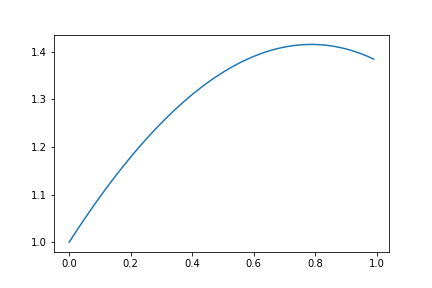
\includegraphics[width = .8 \linewidth]{images/hw05q01b.png}
    \caption{$p_3(x)$ vs $f(x)$}
    \label{fig:my_label}
\end{figure}

\subsection*{(b)}

\begin{align*}
    |F| &\le \frac{(0.5)^4}{4(4)}|F^4(x)| \le \frac{0.5^4}{16}\sqrt{2} = \sqrt{2}\\
    \text{Therefore, the upper bound is $\sqrt{2}$}\\
    f^4(x) &= \sin(x) + \cos(x) \le 1.414\\
\end{align*}


\section{}
Let $f: [-1,1] \to \mathbb{R}$ be continuous.
\begin{enumerate}[label = (\alph*)]
    \item Construct a Lagrange interpolation polynomial $p_1 \in P_1$ for $f$ using the interpolation points $x_0 = -1$ and $x_1 = 1$.
    \item Show further that if $f \in C^2([-1,1], \mathbb{R})$ then $$|f(x)-p_1(x)| \le \frac{M_2}{2}(1-x^2) \le \frac{M_2}{2},$$
    for all $x \in [-1,1]$, where $M_2 = \underset{x \in [-1,1]}{max} |f''(x)|$.
    \item Give an example of $f$, and a point $x$, for which
    $$|f(x)-p_1(x)|= \frac{M_2}{2}(1-x^2)$$
\end{enumerate}
\vspace{10mm}

\subsection*{(a)}
\begin{align*}
    x_0 &= -1 \quad x_1=1\\
    p_1(x) &= \sum_{k=0}^n f(x_k) \cdot L_k(x) \\
    &= \sum_{k=0}^n f(x_k) \prod_{i=k=0}^{n} \frac{x-x_i}{x_k - x_i}\\
    L_0 &=  \frac{x-x_1}{x_0 - x_1} = \frac{x-1}{-1-1} =\frac{x-1}{-2}\\
    L_1 &=   \frac{x-x_0}{x_1 - x_0} = \frac{x-(-1)}{1-(-1)} =\frac{x+1}{2}\\
    p_1(x) &= f(-1) \frac{x-1}{-2}+ f(1) \frac{x+1}{2} = \frac{f(-1)(x-1)}{-2}+  \frac{f(-1)(x+1)}{2}
\end{align*}

\subsection*{(b)}

\begin{align*}
    M_2 &= \underset{x \in [-1,1]}{max} |f''(x)| \\
    &= \prod_{i=0}^1 (|x-x_i|) = |(x-x_0)(x-x_1)| = |(x-(-1))(x-1)|\\
    &= |(x-1)(x+1)| = |x^2-1|=1-x^2\\
    |f(x)-p_1(x)| & \le \frac{M_2}{2}(1-x^2)\\
    1 &= \underset{x \in [-1,1]}{max} |1-x^2| \\
    |f(x)-p_1(x)| & \le \frac{M_2}{2}(1-x^2) \le \frac{M_2}{2}\\
\end{align*}

\subsection*{(c)}
\begin{align*}
    f(x)&= x^2 \quad x=1 \\
    f'(x) &= 2x \quad f''(x) = 2 \\
    f(1) &= 1 \quad f(-1)=1 \\
    p_1(1) &= \frac{1 \cdot (1+1)}{2} - \frac{1 \cdot (1-1)}{2}=1\\
    |f(1)-p_1(1)| &= |1-1 | =0\\
    0 &= \frac{M_2}{2} (1-1^2)\\
    \text{When $f(x)=x^2$ and $x=1$ then,}&\\
    |f(1)-p_1(1)| &= \frac{M_2}{2} (1-x^2)
\end{align*}

\section{}
\begin{enumerate}[label = (\alph*)]
    \item Write down the Lagrange interpolation polynomial $p_1 \in \mathcal{P}_1$ for the function $f:x \to x^3$, using the points $x_0 = 0$, $x_1 = a$. Verify that Theorem 6.2 [Endre Suli and David Mayers, An Introduction to Numerical Analysis, Cambridge University Press, 2008] holds for this example by direct calculation, showing that in this case $\xi$ is unique and has the value $\xi=\frac{1}{3}(x+a)$.
    \item Repeat the calculation for the function $f: x \to (2x-a)^4$; show that in this case there are two possible values for $\xi$, and state their values.
\end{enumerate}
\vspace{10mm}

\subsection*{(a)}
Theorem 6.2
\begin{equation}\label{thm:6.2a}
    f(x) - p_n(x) = \frac{f^{(n+1)}\xi}{(n+1)!} \pi_{n+1}(x)
\end{equation}
\begin{equation}\label{thm:6.2b}
    \pi_{n+1}(x) = (x-x_0) \dots(x-x_n)
\end{equation}
\begin{align*}
    f(x) &= x^3 \quad f'(x)=3x^2 \quad f''(x) = 6x \\
    L_0 &=  \frac{x-x_1}{x_0 - x_1} = \frac{x-a}{0-a} =\frac{x-a}{-a}\\
    L_1 &=   \frac{x-x_0}{x_1 - x_0} = \frac{x-0}{a-0} =\frac{x}{a}\\
    x^3 - a^2x &= \frac{f^2(\xi)}{2!}(x-0)(x-a)\\
    (x)(x-a)(x+a) &= \frac{6 \xi}{2}(x-0)(x-a)\\
    (x+a) &= \frac{6 \xi}{2}\\
    \xi &= \frac{2(x+a)}{6} = \frac{1}{3}(x+a)
\end{align*}

\subsection*{(b)}

\begin{align*}
    f(x) &=(2x-a)^4 \quad f'(x)= 8(2x-a)^3 \quad f''(x) = 48(2x-a)^2\\
    f(0) &= a^4 \quad f(a)=a^4\\
    L_0 &= \frac{x-a}{a} \quad L_1 = \frac{x}{a}\\
    \pi_2 &=(x-0)(x-a) = x^2-ax\\
    p_1(x) &= f(0) \frac{x-a}{a} + f(a) \frac{x}{a}\\
    &= a^4 \frac{x-a}{a} + a^4 \frac{x}{a}\\
    p_1(x) &= a^3(x-a) + a^3(x)\\
    f(x) &= P_n(x) = \frac{f^{(n+1)}(\xi)}{(n+1)!}\pi_{(n+1)}(x)\\
    (2x-a)^4 - p_1 &= \frac{f''(\xi)}{2!}\pi_2(x)\\
    (2x-a)^4 - a^4 &= \frac{48(2x-a)^2}{2}(x^2-ax)\\
    \xi &= \pm \sqrt{\frac{(2x-a)^4-a^4}{24(x^2-ax)}}+\frac{a}{2}
\end{align*}

\section{}
 Given the distinct points $x_i$, $i = 0, 1,\dots, n + 1$, and the points $y_i$, $i = 0, 1, \dots , n + 1$, let $q$ be the Lagrange polynomial of degree $n$ for the set of points $\{(x_i, y_i) : i = 0, 1, \dots` , n\}$ and $r$ be the Lagrange polynomial of degree $n$ for the points $\{(x_i, y_i) : i = 1,\dots, n + 1\}$. Define
 \begin{equation*}
     p(x) = \frac{(x-x_0)r(x)-(x-x_{n+1}q(x))}{x_{n+1}-x_0}.
 \end{equation*}
 Show that $p$ is the Lagrange polynomial of degree $n+1$ for the points $\{(x_i,y_i): i =0,1,\dots, n+1 \}$.
\vspace{10mm}





\end{document}